\DocumentMetadata{lang=en-US, testphase=phase-III}
\documentclass{article}
\usepackage[letterpaper, margin=1in]{geometry}
\usepackage[T1]{fontenc}
\usepackage{tgtermes}
\usepackage{graphicx}
\usepackage{caption}
\usepackage{subcaption}
\usepackage{hyperref}
\graphicspath{{photos/}{figures/}}

\title{Data Analytics Workshop Discussion 2}
\author{Aaron Zoll}
\date{}

\begin{document}
\maketitle

\section*{Introduction}
Below you will see two images, one of some fireworks I took at my camp and another of a building on campus.

\begin{figure}[h]
  \centering
  \begin{subfigure}{0.5\textwidth}
    \centering
    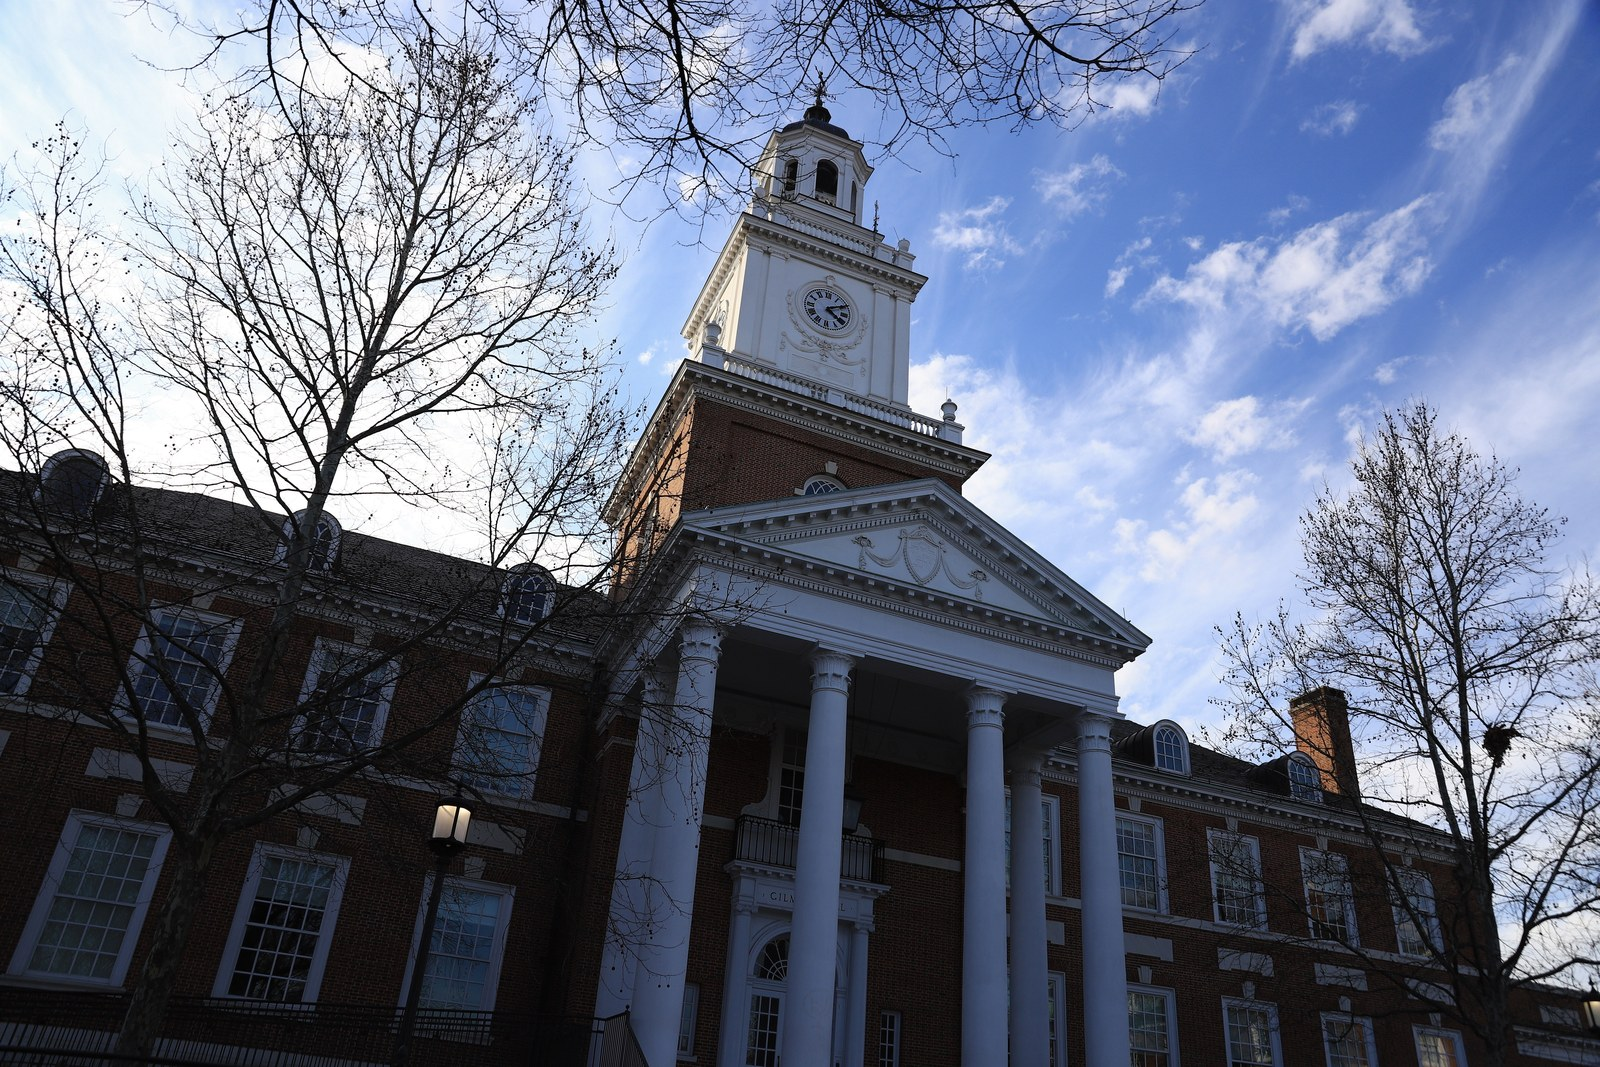
\includegraphics[width=0.95\linewidth, alt={Color photo of Gilman Hall, a brick building with a clock tower, under a blue sky.}]{gilman.jpg}
    \caption{Gilman}
  \end{subfigure}%
  \begin{subfigure}{0.5\textwidth}
    \centering
    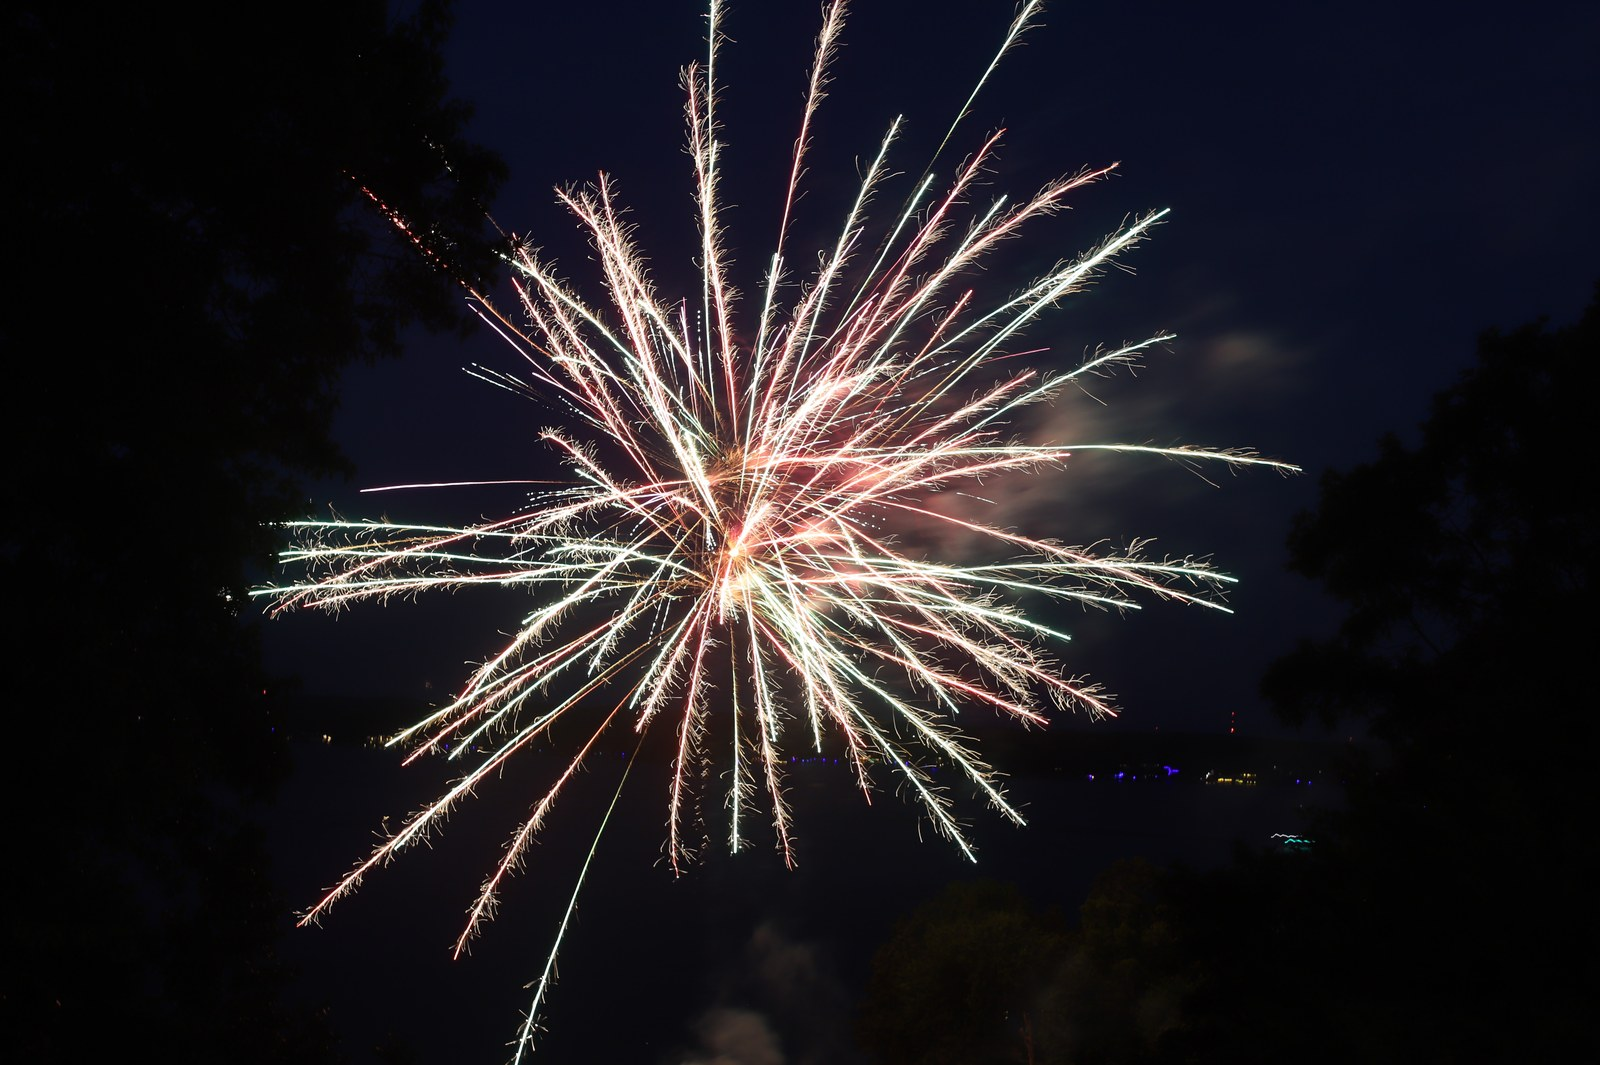
\includegraphics[width=0.95\linewidth, alt={Color photo of a white and pink firework bursting against a black night sky.}]{fireworks.jpg}
    \caption{Fireworks}
  \end{subfigure}
\end{figure}

These pictures are saved as a common file type for images: JPEG (``.jpg''). This means the data for each image is stored pixel by pixel, with three numbers ranging from $0$ to $255$ for the red, green, and blue components. If we just look at the red components of each image, we get a new image, now with each pixel having a range from $0$ to $255$, where we can consider this just a brightness. From this image we can plot a black-and-white version, with $0$ being a purely black pixel, $255$ being a purely white pixel, and anything in between corresponding to different grey values.

\begin{figure}[h]
  \centering
  \begin{subfigure}{0.5\textwidth}
    \centering
    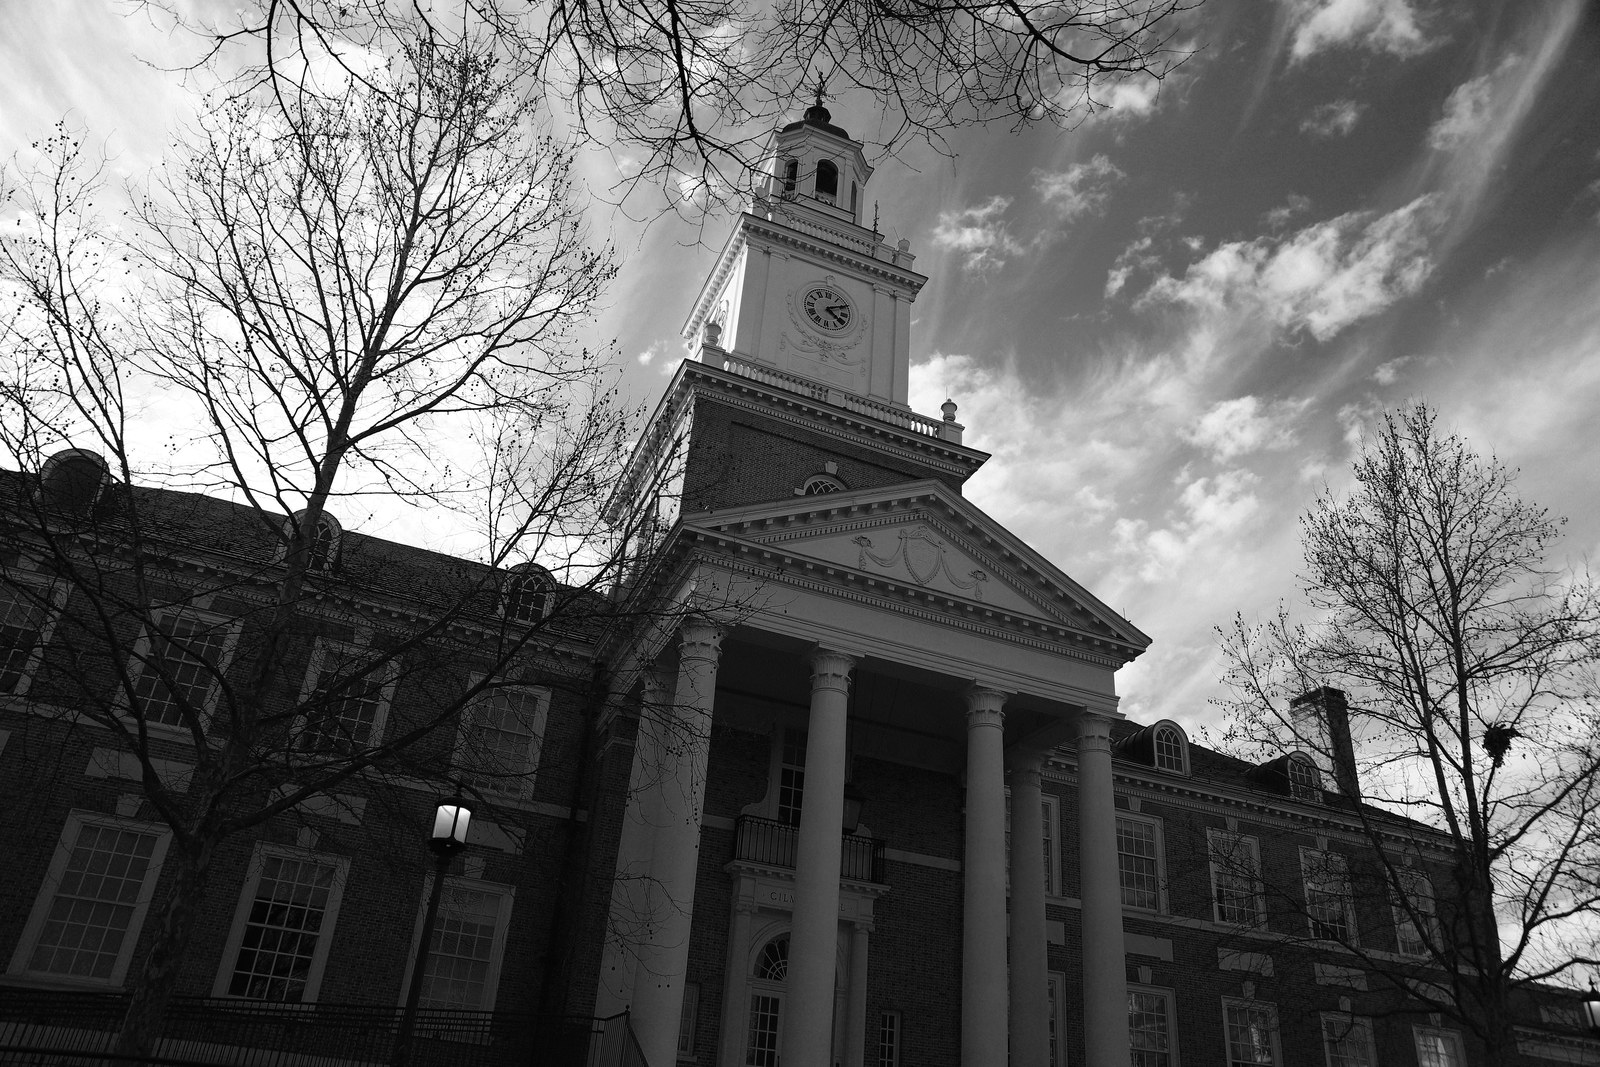
\includegraphics[width=0.95\linewidth, alt={Black-and-white version of the Gilman photo made from its red component.}]{gilman_red.jpg}
    \caption{Gilman black-and-white}
  \end{subfigure}%
  \begin{subfigure}{0.5\textwidth}
    \centering
    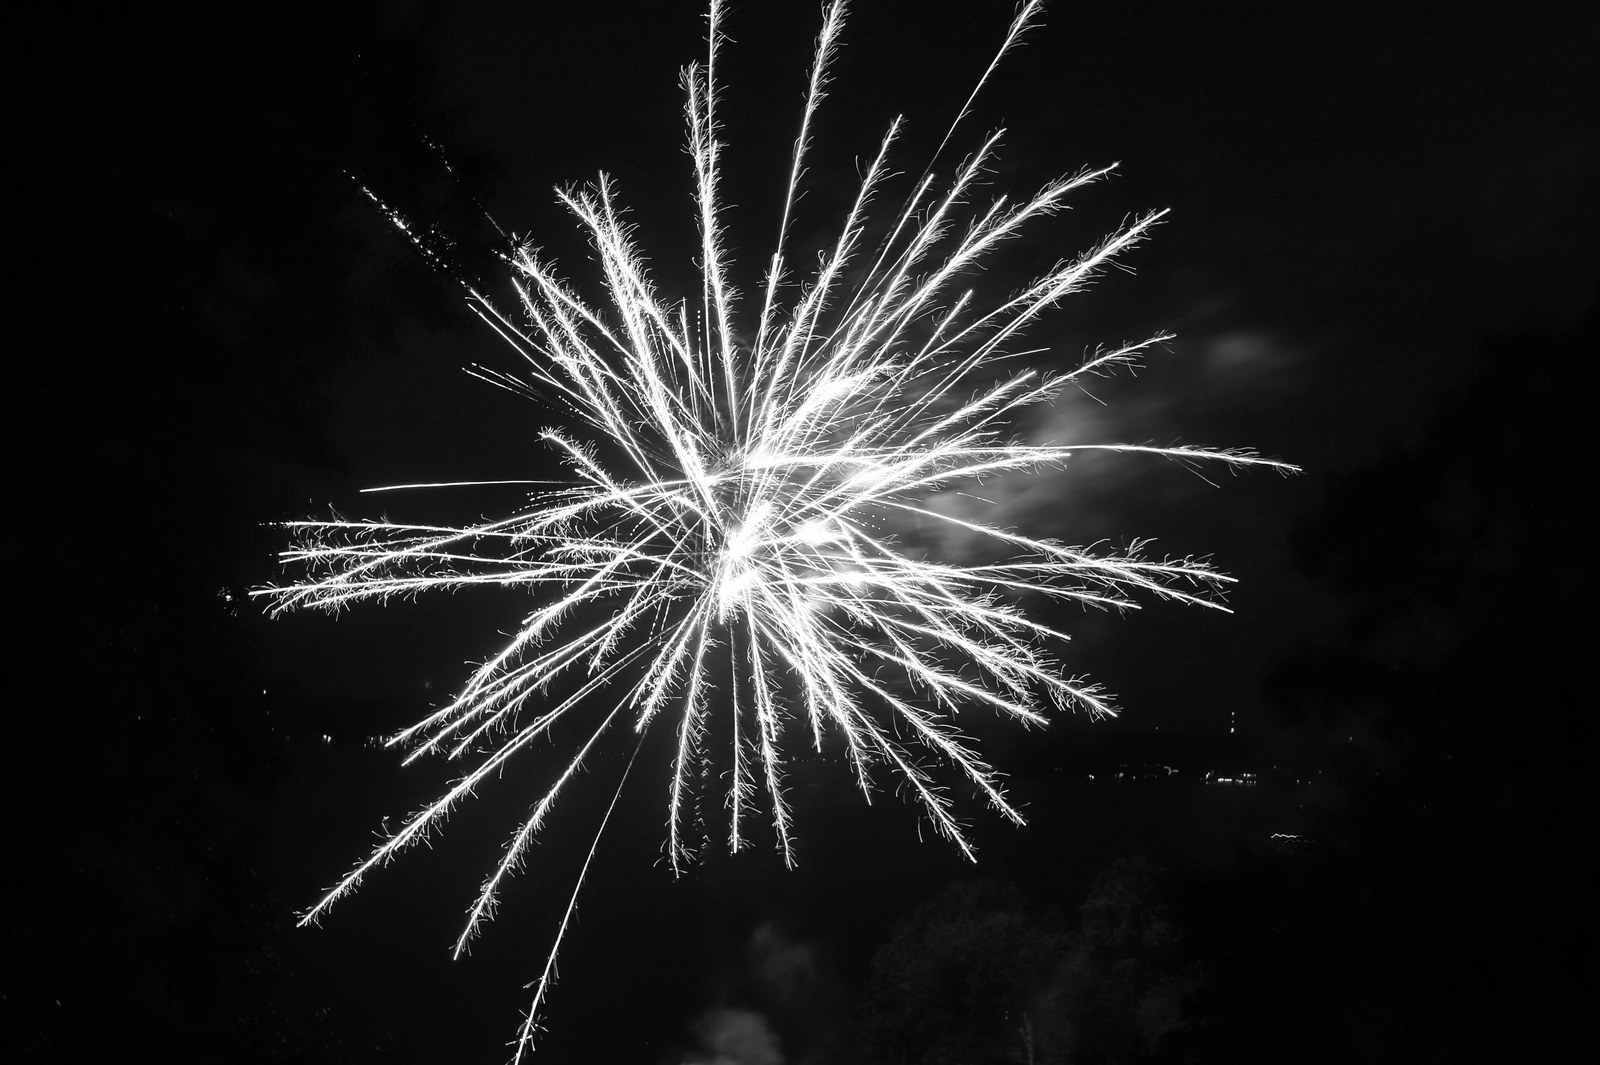
\includegraphics[width=0.95\linewidth, alt={Black-and-white version of the fireworks photo made from its red component.}]{fireworks_red.jpg}
    \caption{Fireworks black-and-white}
  \end{subfigure}
\end{figure}

To make the plots in this worksheet, each photo was shrunk to $300 \times 200$ pixels, so each image has $60{,}000$ pixels.

\clearpage
\section*{Histograms}
Below you will see two sets of histograms for the black-and-white images. The way histograms work is by taking the amount of data that falls into a certain range and plotting that. For example, the first histogram tells us there are about $16{,}500$ pixels in the black-and-white fireworks picture that have brightness anywhere from $0$ to $4$. We can also read that there are around $50{,}000$ pixels that have brightness $0$ to $54$ from the top histogram on the right. Finally, we have about $4{,}800$ pixels with brightness of $220$ to $255$ in the Gilman photo, as noted by the last bar in the bottom right histogram.

Note that in the first column we have a histogram with thinner bins. That is, when clumping the data together, we take note of a smaller range. This gives us finer detail and more information. Finally, note that by adding the sizes of narrower bins together, we can perfectly recreate the wider bins, but we cannot do the reverse (e.g. adding the first $11$ bin sizes in one of the left histograms gives us the size of the first bin in the right histogram).

\begin{figure}[h]
  \centering
  \begin{subfigure}{0.5\textwidth}
    \centering
    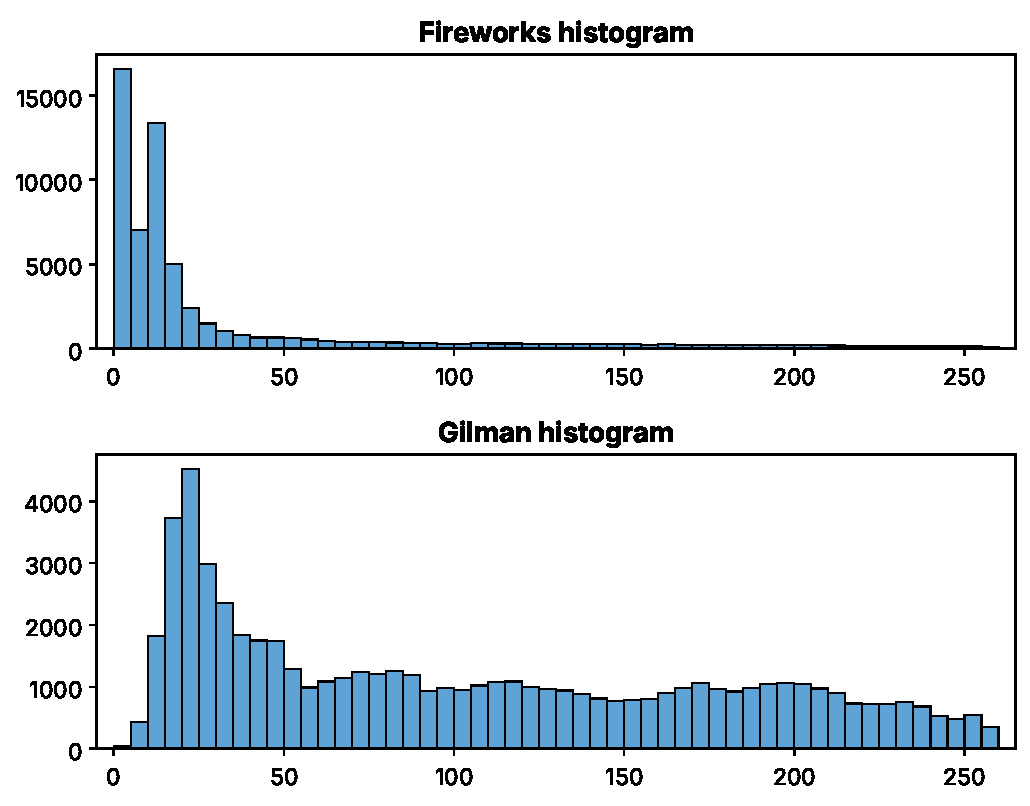
\includegraphics[width=0.95\linewidth, alt={Histograms of pixel brightness with bins of width 5. Fireworks: a tall spike near 0 and very few bright pixels. Gilman: a peak near 25, then roughly level counts out to 255.}]{hist_narrow.pdf}
  \end{subfigure}%
  \begin{subfigure}{0.5\textwidth}
    \centering
    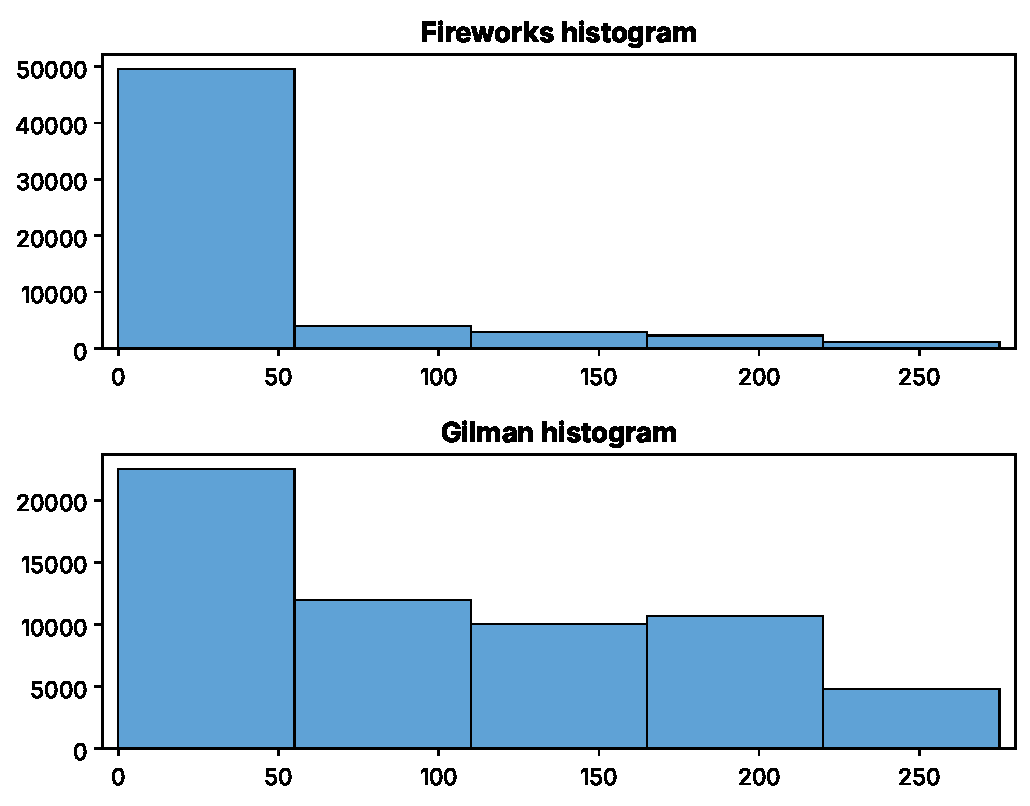
\includegraphics[width=0.95\linewidth, alt={Histograms of pixel brightness with bins of width 55. Fireworks: about 50,000 pixels in the first bin and a few thousand in each other bin. Gilman: about 22,500 in the first bin, 10,000 to 12,000 in the middle three, and about 4,800 in the last.}]{hist_wide.pdf}
  \end{subfigure}
\end{figure}

\clearpage
\section*{Bar charts}
Here we have bar charts that plot the average intensity of each color in the two pictures. Recall that each picture is originally in color, and so each pixel has a red, green, and blue intensity. We can average the intensity of all the pixels to figure out how much of the picture is red, green, or blue. Examine the bar charts below and draw some conclusions about the images. Does this match with what you see visually? (Note: each pixel has three components: red, green, and blue. If those three components are evenly leveled, the pixel is grey. The bar charts show the average intensity among all the pixels, so if the bars are relatively even, we have two options. Either the components are relatively even for each pixel, in which case we should see a lot of grey, black, and white, or there is about as much ``blue section'' in the image as ``red section'' or ``green section.'' If one pixel has intensities $(30, 60, 90)$ and another has $(60, 120, 180)$, they will be the same hue (color) because the ratios are the same, but the second will be brighter.)

\begin{figure}[h]
  \centering
  \begin{subfigure}{0.5\textwidth}
    \centering
    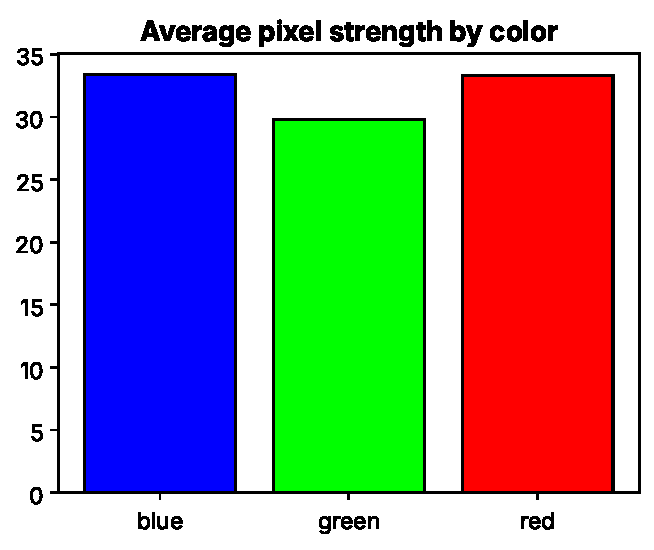
\includegraphics[width=0.95\linewidth, alt={Bar chart of average pixel strength: blue about 33, green about 30, red about 33.}]{bar_fireworks.pdf}
  \end{subfigure}%
  \begin{subfigure}{0.5\textwidth}
    \centering
    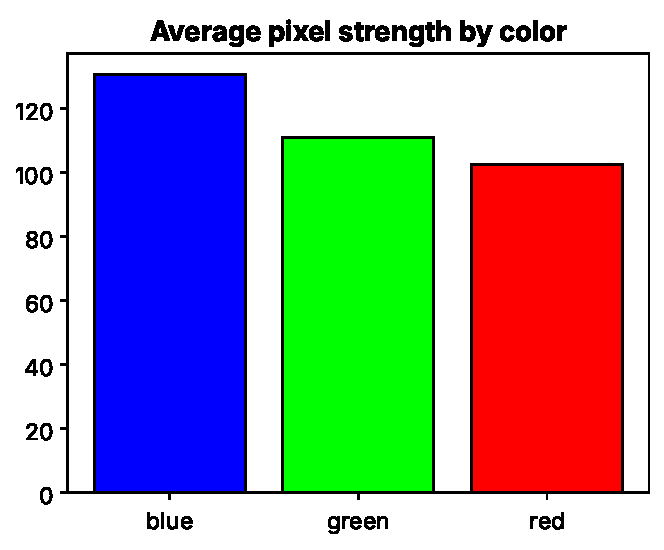
\includegraphics[width=0.95\linewidth, alt={Bar chart of average pixel strength: blue about 131, green about 111, red about 102.}]{bar_gilman.pdf}
  \end{subfigure}
\end{figure}

Here are the three components of each image, only showing the blue, green, and red components. See if and how these align with the charts above. Also note the difference in magnitudes of the values in the left and right bar charts. Which graph do you think represents which image?

\begin{figure}[h]
  \centering
  \begin{subfigure}{0.33\textwidth}
    \centering
    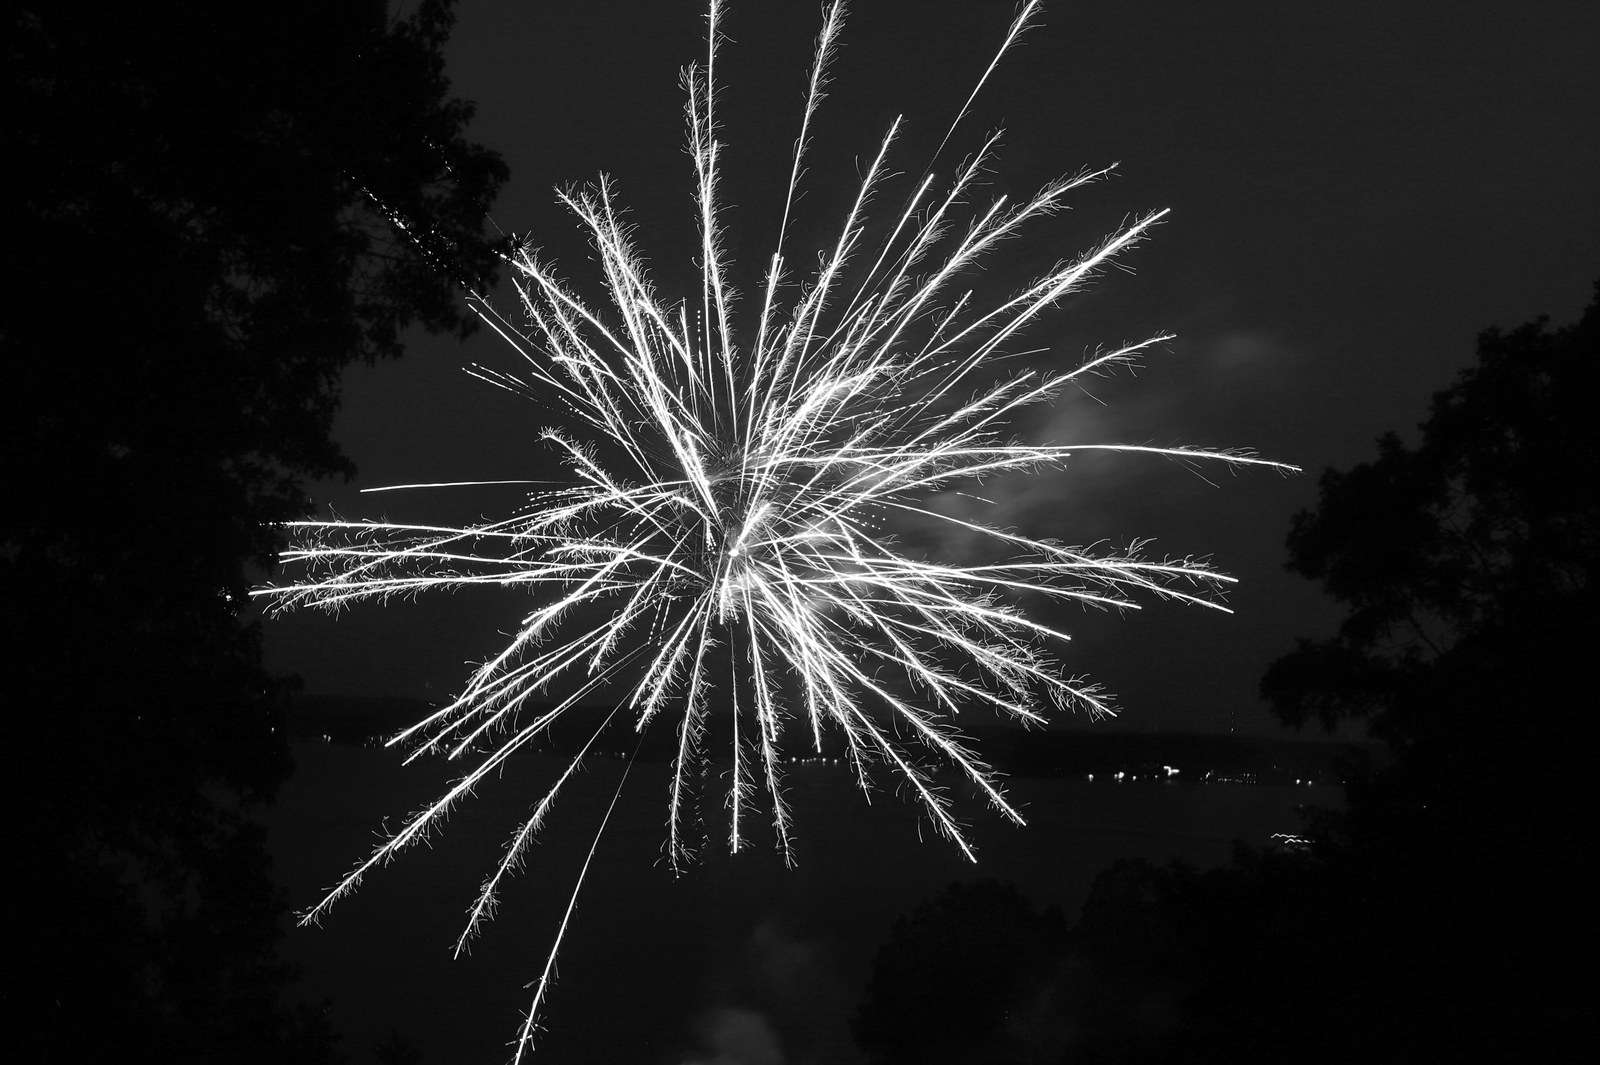
\includegraphics[width=0.95\linewidth, alt={Blue component of the fireworks photo shown in greyscale.}]{fireworks_blue.jpg}
    \caption{blue component}
  \end{subfigure}%
  \begin{subfigure}{0.33\textwidth}
    \centering
    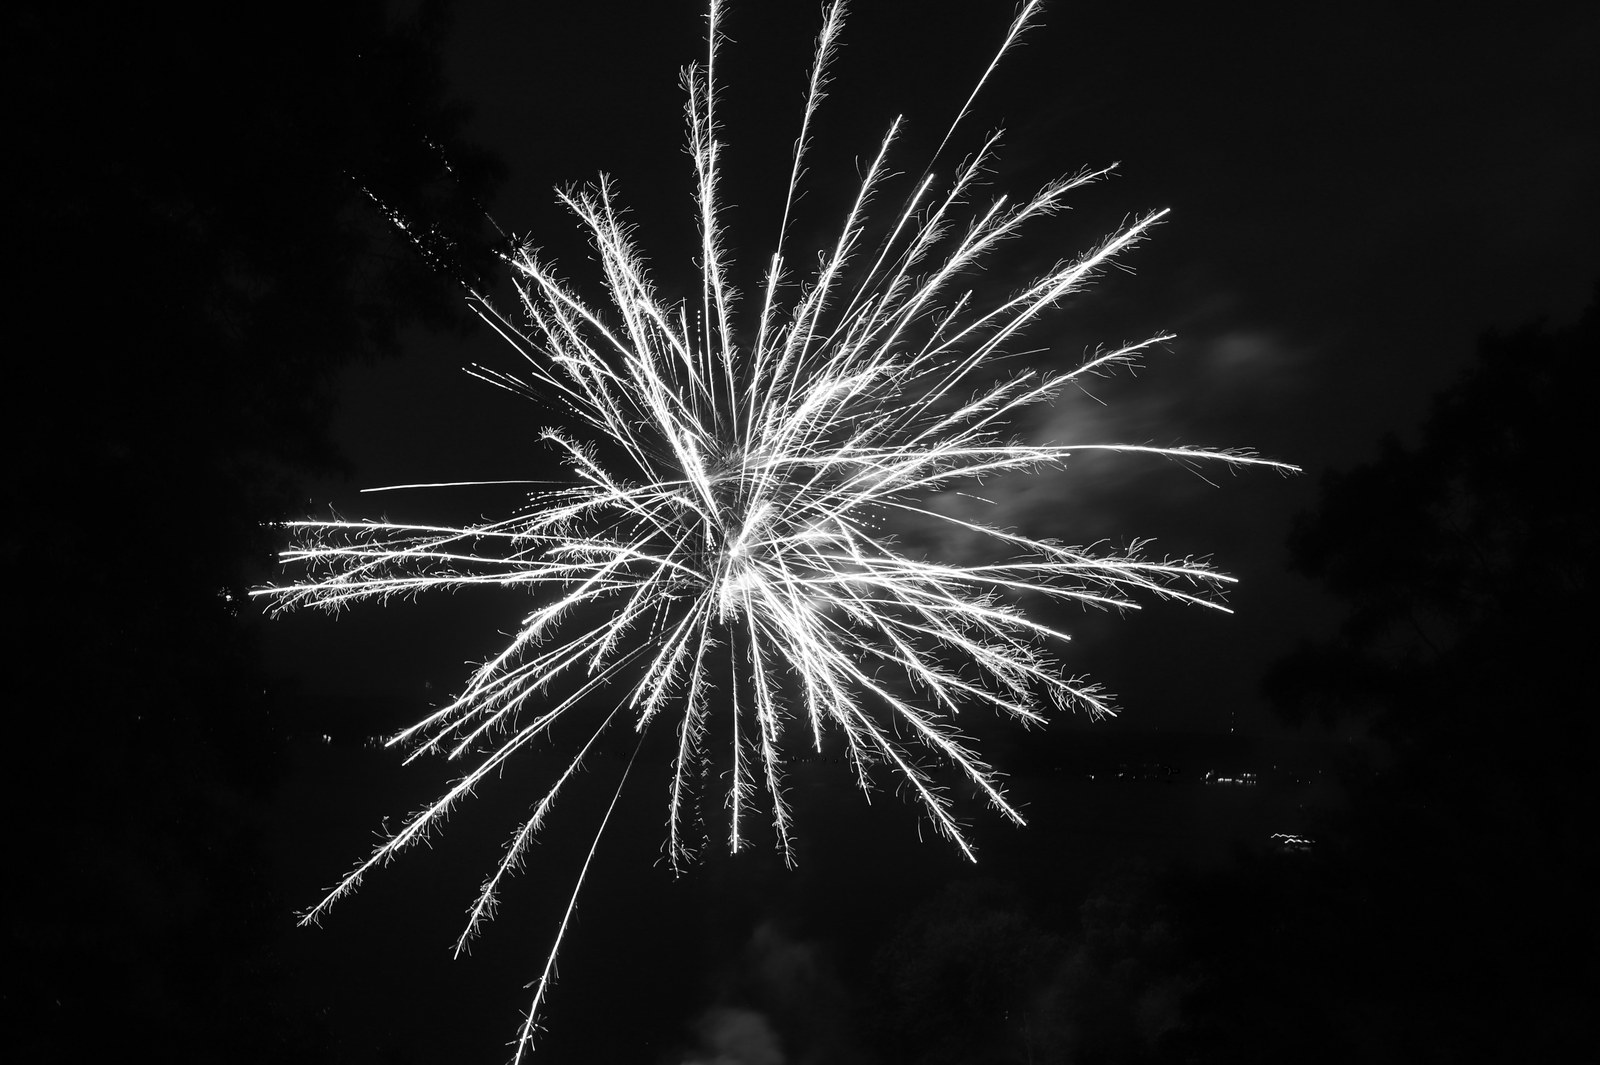
\includegraphics[width=0.95\linewidth, alt={Green component of the fireworks photo shown in greyscale.}]{fireworks_green.jpg}
    \caption{green component}
  \end{subfigure}%
  \begin{subfigure}{0.33\textwidth}
    \centering
    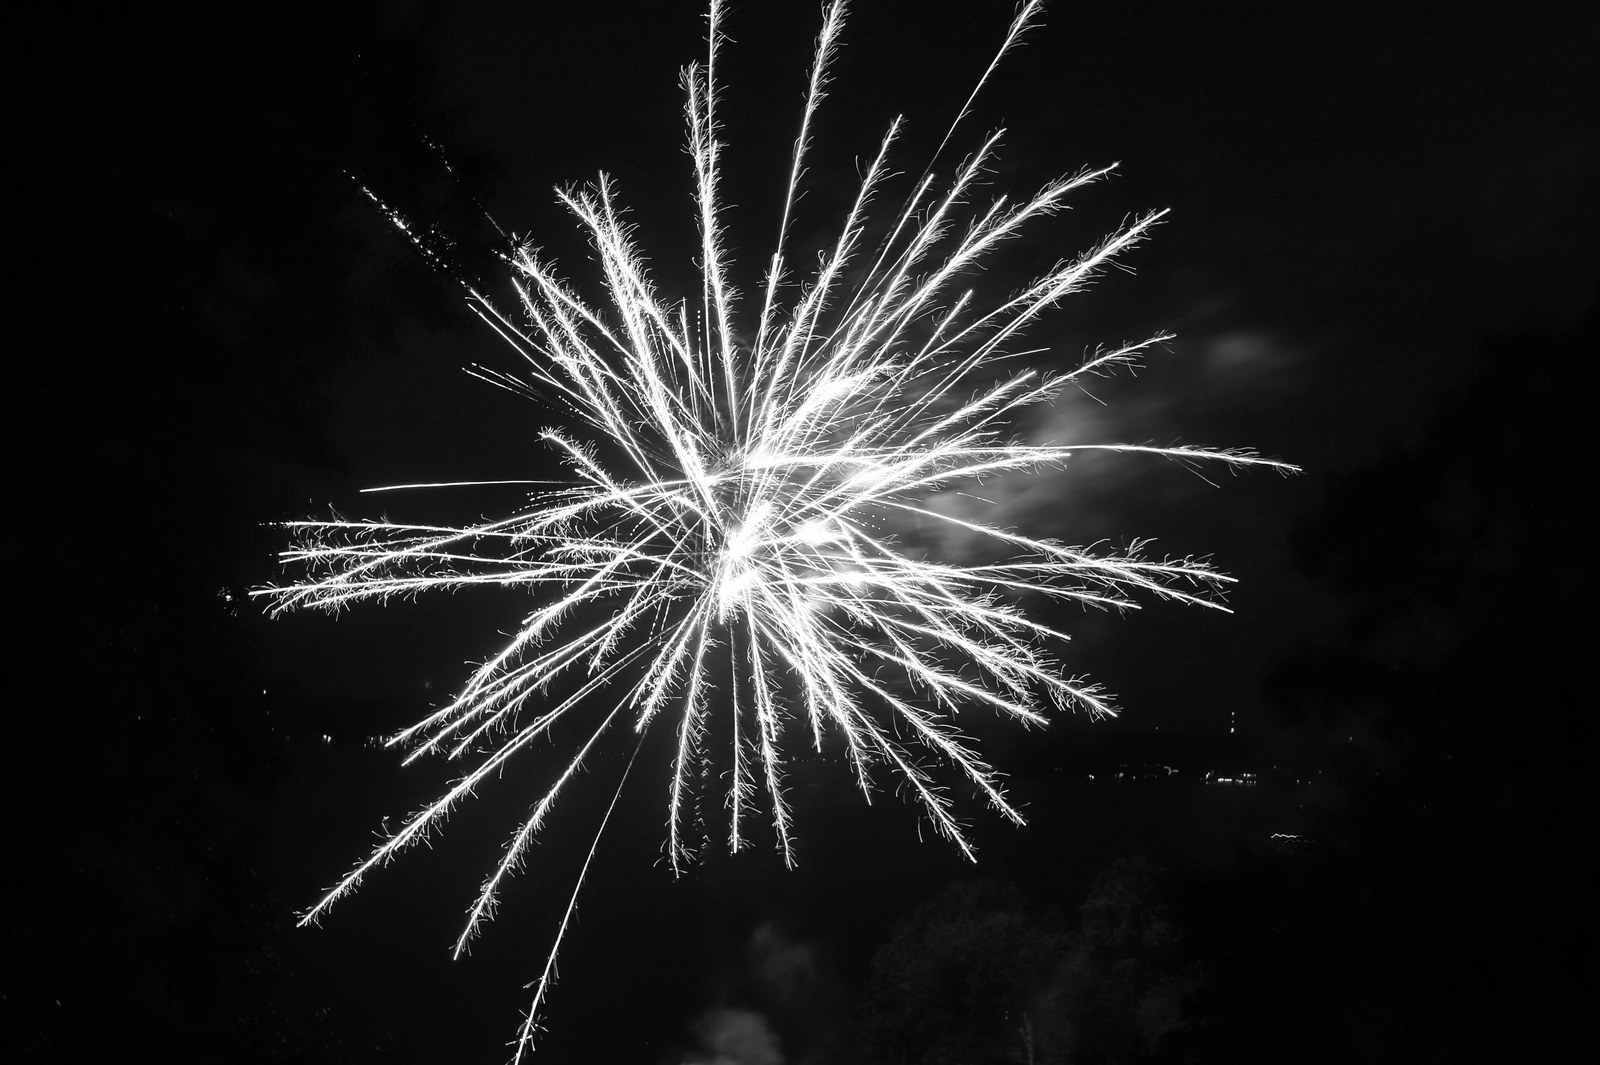
\includegraphics[width=0.95\linewidth, alt={Red component of the fireworks photo shown in greyscale.}]{fireworks_red.jpg}
    \caption{red component}
  \end{subfigure}
\end{figure}

\begin{figure}[h]
  \centering
  \begin{subfigure}{0.33\textwidth}
    \centering
    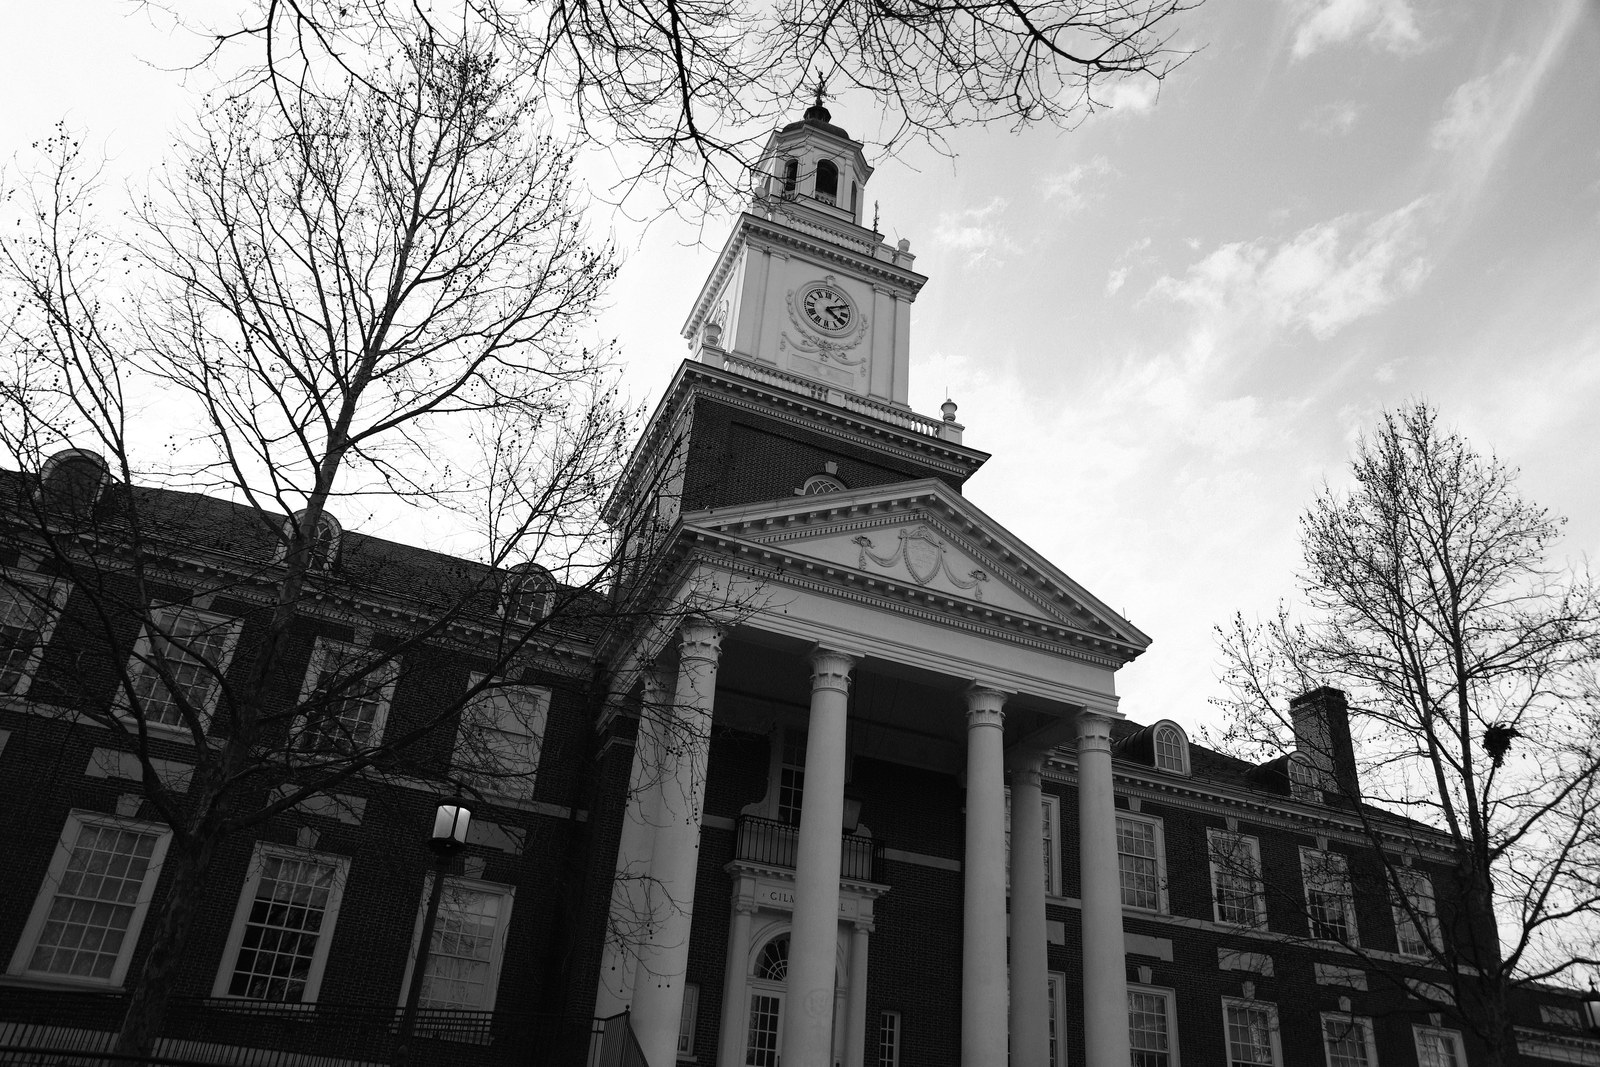
\includegraphics[width=0.95\linewidth, alt={Blue component of the Gilman photo shown in greyscale. The sky is bright.}]{gilman_blue.jpg}
    \caption{blue component}
  \end{subfigure}%
  \begin{subfigure}{0.33\textwidth}
    \centering
    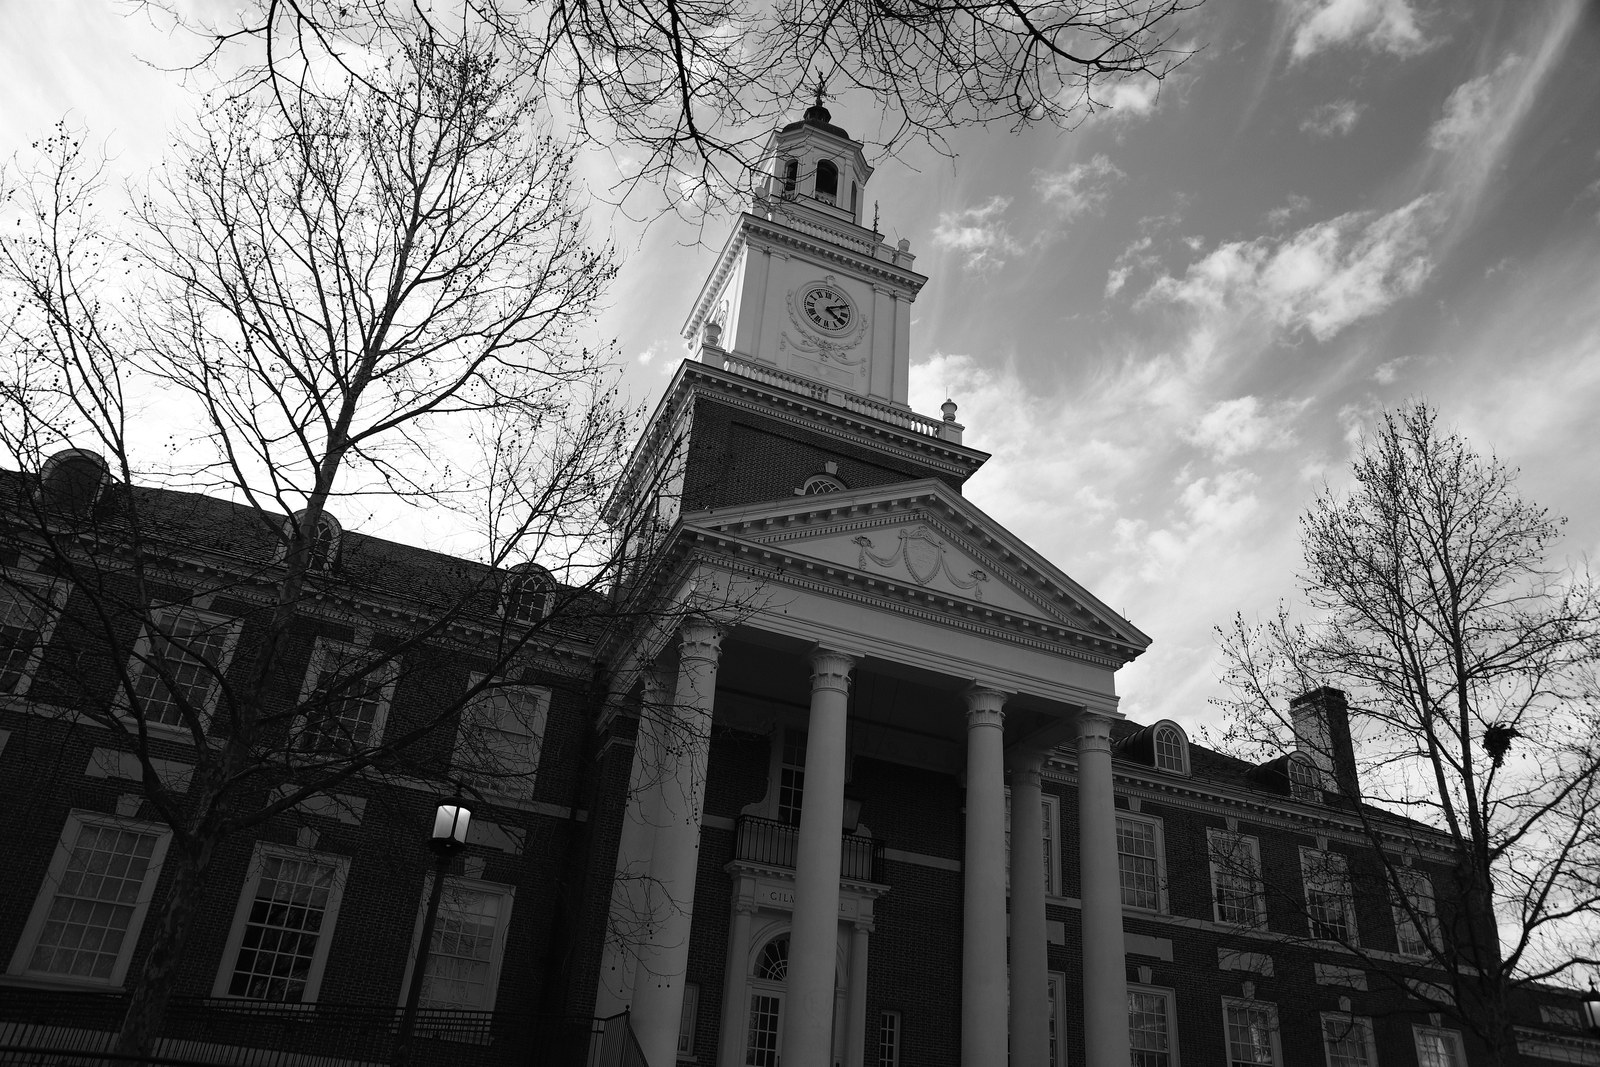
\includegraphics[width=0.95\linewidth, alt={Green component of the Gilman photo shown in greyscale.}]{gilman_green.jpg}
    \caption{green component}
  \end{subfigure}%
  \begin{subfigure}{0.33\textwidth}
    \centering
    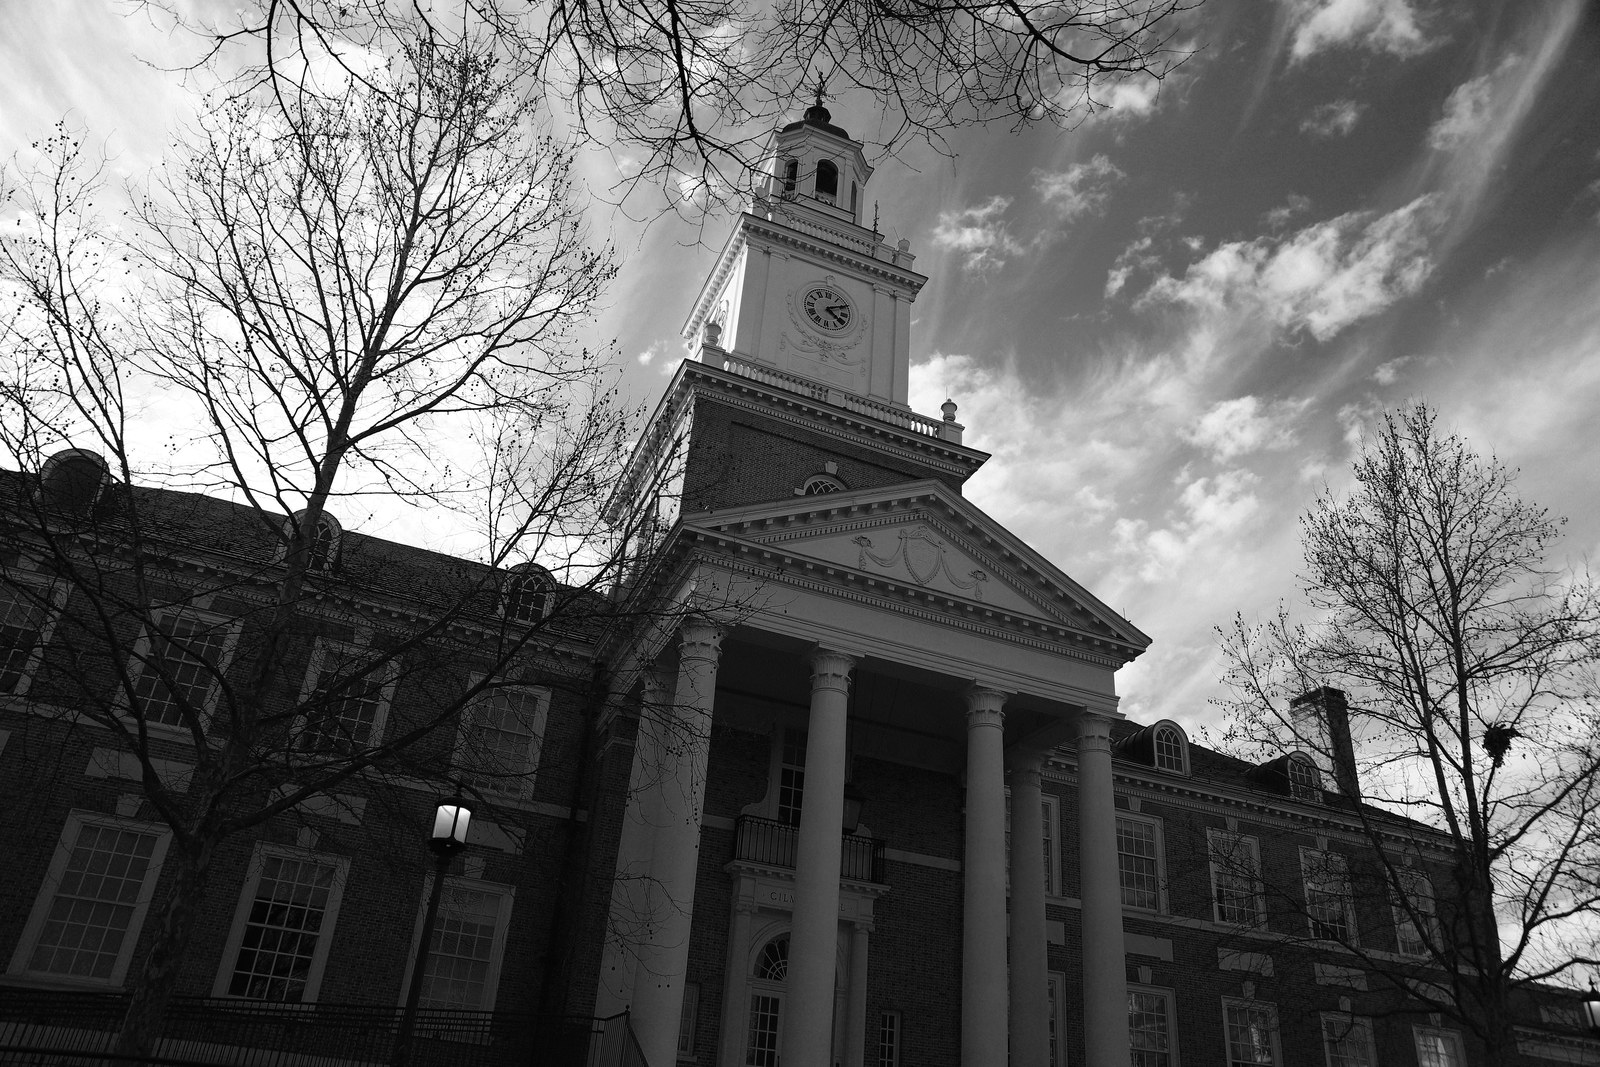
\includegraphics[width=0.95\linewidth, alt={Red component of the Gilman photo shown in greyscale. The sky is darker than in the blue component.}]{gilman_red.jpg}
    \caption{red component}
  \end{subfigure}
\end{figure}

\clearpage
\section*{Scatter plots}
Consider the two pictures below. Here we are going to try and see how the intensity of one color correlates to the intensity of another. That is, for example, how much can we say a rise in green intensity for a pixel comes with a rise in blue intensity? Notice that one image has very distinct colors, while the Gilman photo does have some color, but it is less rigid and separated.

\begin{figure}[h]
  \centering
  \begin{subfigure}{0.4\textwidth}
    \centering
    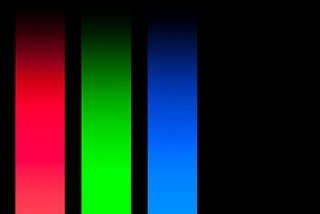
\includegraphics[width=0.95\linewidth, alt={Image of three vertical bars on black: red, green, and blue, each fading from dark at the top to bright at the bottom.}]{colors.jpg}
  \end{subfigure}%
  \begin{subfigure}{0.4\textwidth}
    \centering
    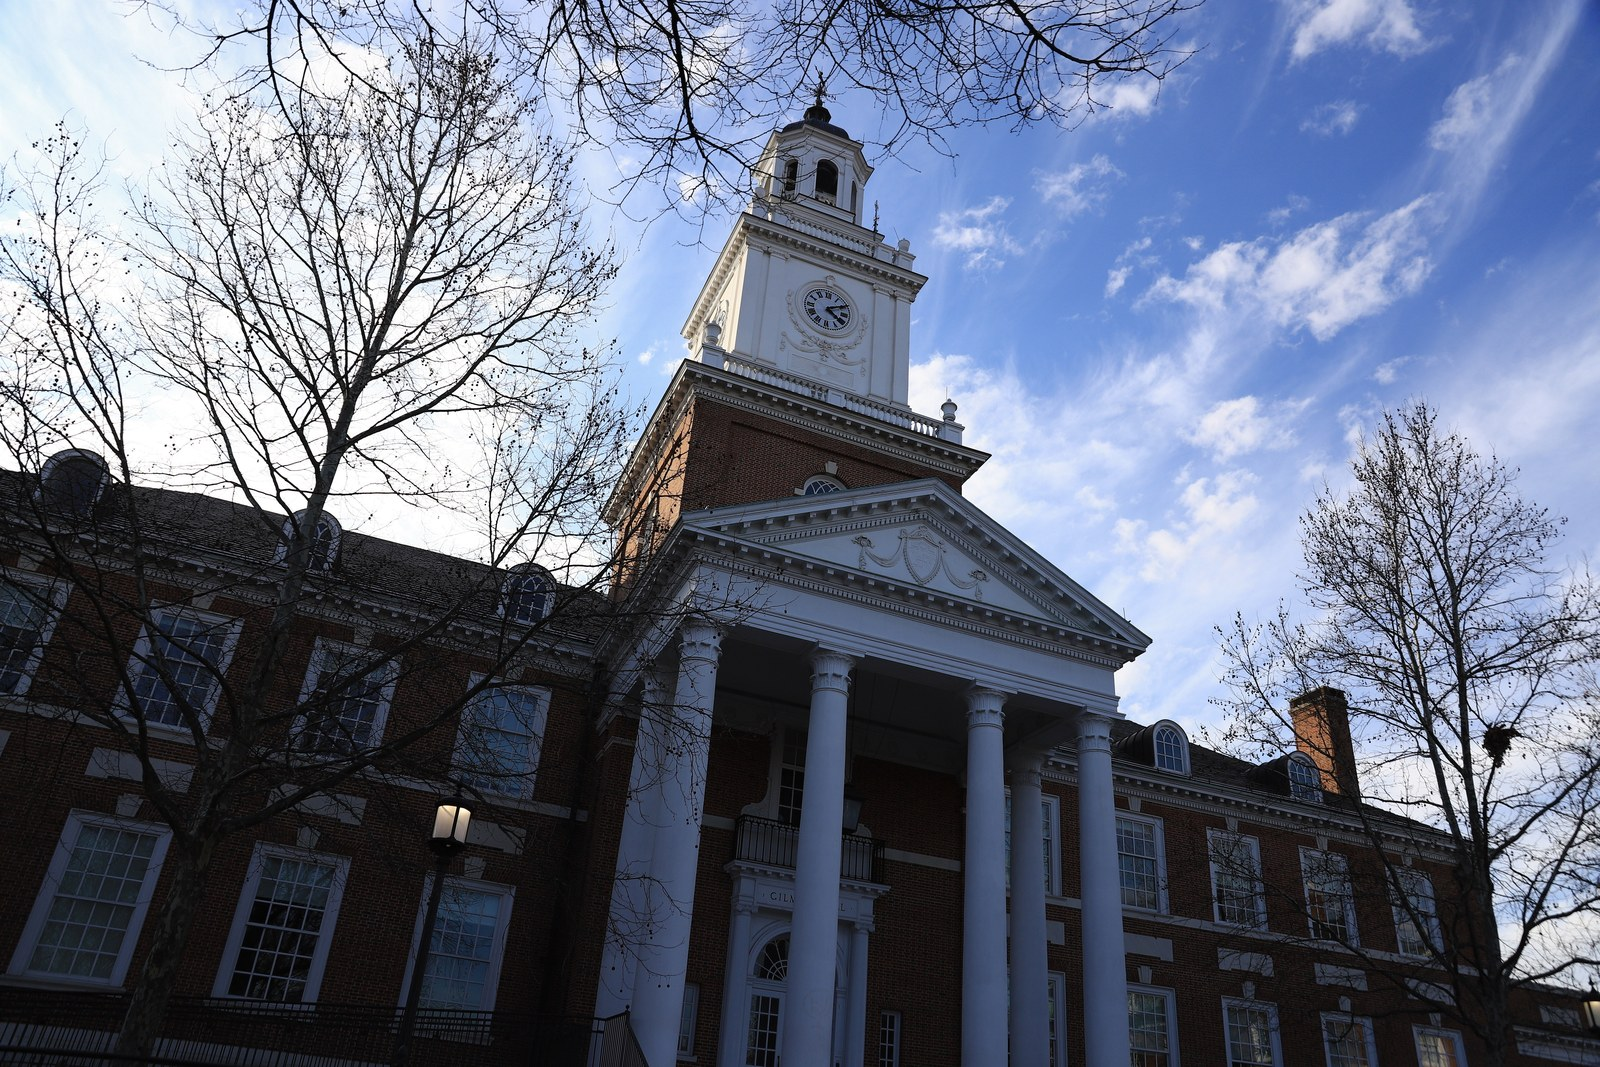
\includegraphics[width=0.95\linewidth, alt={Color photo of Gilman Hall.}]{gilman.jpg}
  \end{subfigure}
\end{figure}

Below are two sets of scatter plots that graph one color intensity versus another for $300$ randomly chosen pixels in each of the two pictures. Notice how for the image with separated colors, we have these ``L'' shapes. In the Blue vs Green graph for the first image, notice that there are some elements to suggest that as the green intensity increases, so does the blue. This may indicate that the green or blue shown are not pure green or pure blue, in the sense that there may be some blue components making up the green section or vice versa. What do you think strong correlation indicates for these photos?

\begin{figure}[h]
  \centering
  \begin{subfigure}{0.3\textwidth}
    \centering
    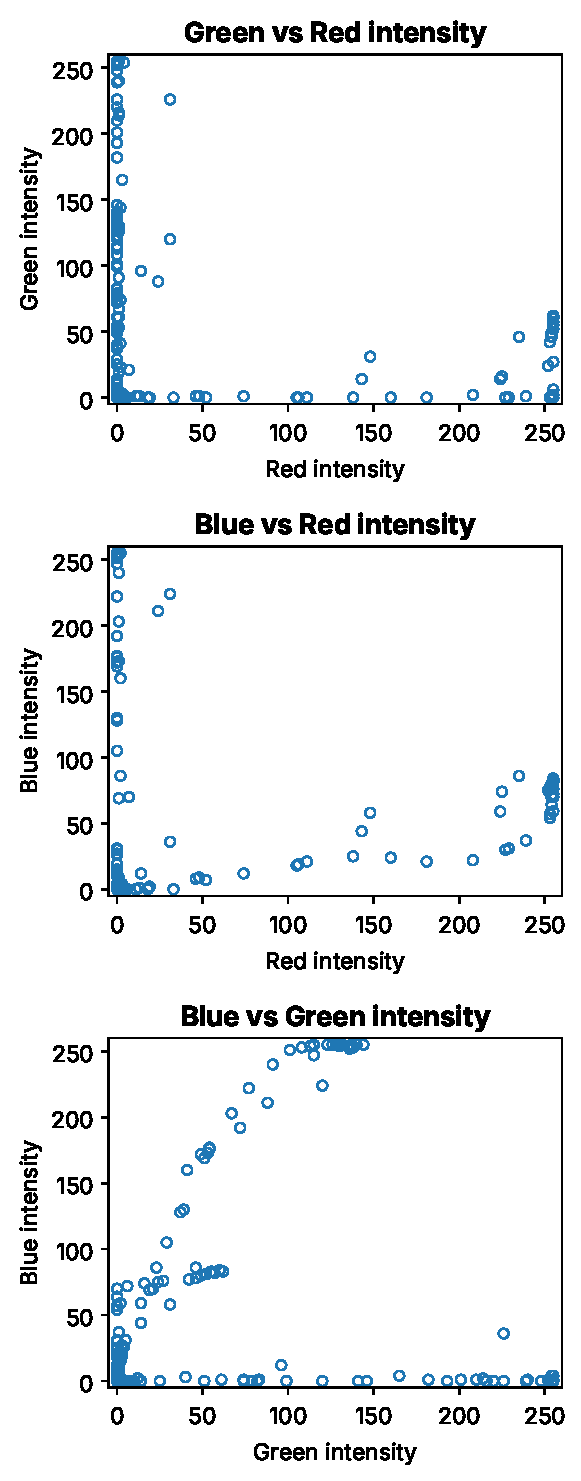
\includegraphics[width=0.95\linewidth, alt={Three scatter plots for the color-bar image. Green vs Red and Blue vs Red form L shapes along the axes. Blue vs Green has an L shape plus curved arcs where blue rises with green.}]{scatter_colors.pdf}
  \end{subfigure}%
  \begin{subfigure}{0.3\textwidth}
    \centering
    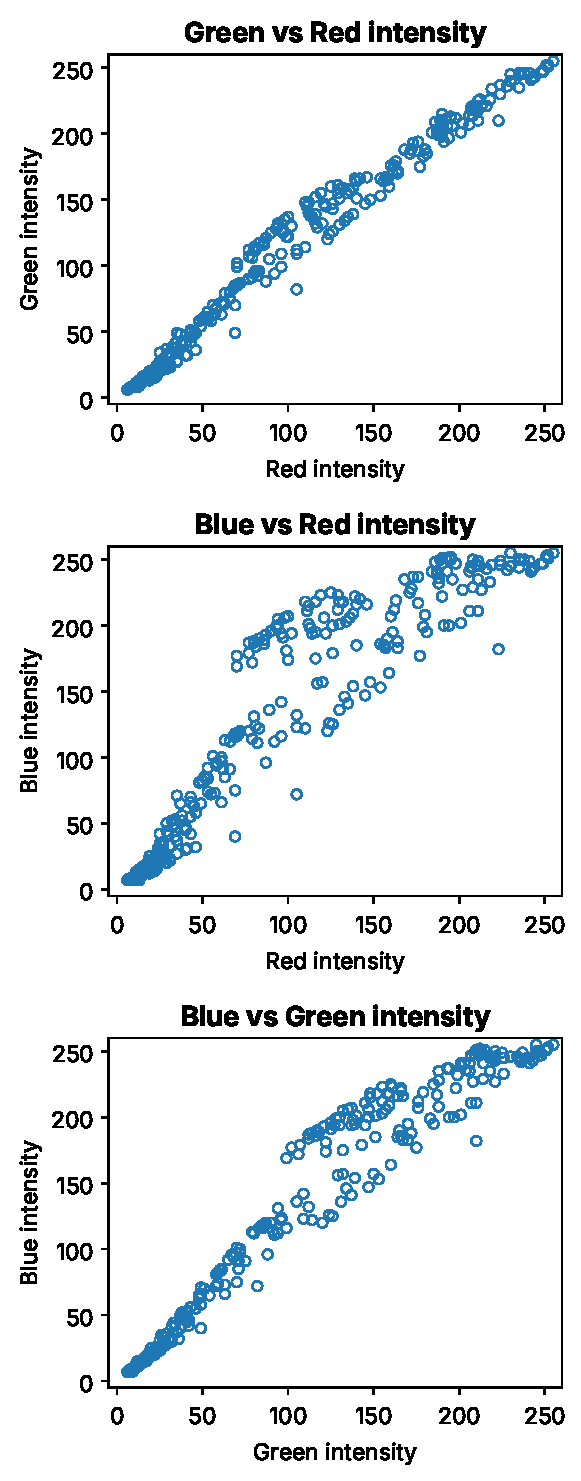
\includegraphics[width=0.95\linewidth, alt={Three scatter plots for the Gilman photo. In each, the points lie close to a rising straight line.}]{scatter_gilman.pdf}
  \end{subfigure}
\end{figure}

\end{document}
